\documentclass[11pt,letterpaper]{article}
\usepackage[lmargin=1in,rmargin=1in,bmargin=1in,tmargin=1in]{geometry}
\usepackage{style/quiz}
\usepackage{style/commands}

\usepackage{cancel} 	% Use Cancels

% -------------------
% Content
% -------------------
\begin{document}
\thispagestyle{title}

% Quiz 1
\quizsol \textit{True/False}: The integer 45 has prime factorization $45= 3 \cdot 15$, which shows that 3 and 15 are divisors of 45. Furthermore, we know that 1 is a multiple of 45. \pspace

\sol The statement is \textit{false}. While it is true that $45= 3 \cdot 15$ is a \textit{factorization} of 45, it is not a \textit{prime factorization} of 45 because $15= 3 \cdot 5$. The prime factorization of 45 is $45= 3^2 \cdot 5$. It is true that if $45= 3 \cdot 15$, then 3 and 15 are divisors of 45. Finally, while 1 is a divisor of 45 because $45= 45 \cdot 1$, 1 is not a multiple of 45 because there is not an integer $k$ such that $1= 45k$. \pvspace{1.3cm}



% Quiz 2
\quizsol \textit{True/False}: $\dfrac{\frac{2a}{b}}{\frac{4a}{bc}}= 8c$ \pspace

\sol The statement is \textit{false}. We have\dots
	\[
	\dfrac{\;\;\dfrac{2a}{b}\;\;}{\dfrac{4a}{bc}}= \dfrac{2a}{b} \cdot \dfrac{bc}{4a}= \dfrac{\cancel{2} \cancel{a}}{\cancel{b}} \cdot \dfrac{\cancel{b}c}{\cancel{4}^{\,2} \cancel{a}}= \dfrac{c}{2}
	\] \pvspace{1.3cm}



% Quiz 3
\quizsol \textit{True/False}: The expression $\dfrac{(x y^3)^{-2}}{(x^{-3} y^8)^2}$ when fully simplified is $\dfrac{x^4}{y^{22}}$. \pspace

\sol The statement is \textit{true}. We have\dots
	\[
	\dfrac{(x y^3)^{-2}}{(x^{-3} y^8)^2}= \dfrac{x^{-2} y^{-6}}{x^{-6} y^{16}}= \dfrac{x^6}{x^2 y^6 y^{16}}= \dfrac{x^6}{x^2 y^{22}}= \dfrac{x^4}{y^{22}}
	\] \pvspace{1.3cm}



% Quiz 4
\quizsol \textit{True/False}: $\left( \dfrac{(x^2 y^3)^4}{x^{-3} y^8} \right)^{-1/2}= \dfrac{1}{y^2 \sqrt[11]{x^2}}$ \pspace

\sol The statement is \textit{true}. We have\dots
	\[
	\hspace{-1.7cm} \left( \dfrac{(x^2 y^3)^4}{x^{-3} y^8} \right)^{-1/2}= \left( \dfrac{x^{-3} y^8}{(x^2 y^3)^4} \right)^{1/2}= \left( \dfrac{x^{-3} y^8}{x^8 y^{12}} \right)^{1/2}= \left( \dfrac{y^8}{x^3 x^8 y^{12}} \right)^{1/2}= \left( \dfrac{y^8}{x^{11} y^{12}} \right)^{1/2}= \left( \dfrac{1}{x^{11} y^4} \right)^{1/2}= \dfrac{1}{x^{11/2} y^{4/2}}= \dfrac{1}{y^2 \sqrt{x^{11}}}
	\]
Therefore, the quiz statement is false. The quiz statement has $\sqrt[11]{x^2}= x^{2/11}$ instead of $\sqrt{x^{11}}= x^{11/2}$. 



\newpage



% Quiz 5
\quizsol \textit{True/False}: The real number $0.123412341234\ldots$ is a rational number; therefore, one can find integers $a, b$ such that $\frac{a}{b}= 0.123412341234\ldots$. \pspace

\sol The statement is \textit{true}. A rational number is a real number of the form $\frac{a}{b}$, where $a, b$ are integers and $b \neq 0$. Equivalently, a rational number is a real number whose decimal expansion either terminates or repeats. Because the decimal expansion of $0.123412341234\ldots$ repeats, it must be that $0.123412341234\ldots$ is rational. Therefore, there must be integers $a, b$ such that $\frac{a}{b}= 0.123412341234\dots$. In fact, if $N= 0.123412341234\dots$, we have\ldots
	\begin{table}[!ht]
	\centering\small
	\begin{tabular}{rccc}
	& $10000N$ & $=$ & $1234.123412341234\overline{1234}$ \\ 
	$-$ & $N$ & $=$ & $\phantom{123}0.123412341234\overline{1234}$ \\ \hline
	& $9999N$ & $=$ & $1234$ \\[0.1cm]
	& $N$ & $=$ & $\frac{1234}{9999}$
	\end{tabular}
	\end{table} \pvspace{1.3cm}



% Quiz 6
\quizsol \textit{True/False}: Suppose a course has grade components of homework (50\%), quizzes (10\%), a midterm (20\%), and a final (20\%). If you had a 80\% homework average, 75\% quiz average, and received a 60\% on the midterm, then your average is\dots
	\[
	0.50(80\%) + 0.10(75\%) + 0.20(60\%)= 40\% + 7.5\% + 12\%= 59.5\%
	\] 

\sol The statement is \textit{false}. One's course average is a weighted average where each percentage earned is weighted by the components worth. But then\dots
	\[
	\text{Course Average}= \dfrac{\sum w_i x_i}{\sum w_i}= \dfrac{0.50 \cdot 0.80 + 0.10 \cdot 0.75 + 0.20 \cdot 0.60}{0.50 + 0.10 + 0.20}= \dfrac{0.40 + 0.075 + 0.12}{0.80}= \dfrac{0.595}{0.80}= 0.74375
	\] \pvspace{1.3cm}



% Quiz 7
\quizsol \textit{True/False}: The real number $0.1 \cdot 10^3$ is in scientific notation. \pspace

\sol The statement is \textit{false}. A number in scientific notation is a real number in the form $R \cdot 10^n$, where $1 \leq |R| < 10$ and $n$ is an integer. Observe that the given number is of the form $R \cdot 10^n$ with $R= 0.1$ and $n= 3$. But because $R= 0.1 < 1$, this number is not in scientific notation. Correctly written in scientific notation, the number $0.1 \cdot 10^3= 0.1 \cdot 1000= 100$ is $1 \cdot 10^2$. \pvspace{1.3cm}



% Quiz 8
\quizsol \textit{True/False}: The surface area of a box that is open at the top with dimensions 1~ft $\times$ 8~in $\times$ 5~in is $\text{SA}= 12 \cdot 8 + 2(8 \cdot 5) + 2(12 \cdot 5)= 296 \text{ in}^2$. \pspace

\sol The statement is \textit{true}. We know that the surface area of a `box' is $\text{SA}= 2\ell w + 2 \ell h + 2 wh$. Because the box is open at the top, there is no surface area at the top of the box. The top of the box has surface area $\ell w$. But then the surface area of the described box is $\text{SA}= 2\ell w + 2 \ell h + 2 wh - \ell w= \ell w + 2 \ell h + 2 wh$. When one computes lengths, areas, volumes, etc., one need be sure that one is consistent with units. So we either have $\ell= 12 \text{ in}$, $w= 8 \text{ in}$, and $h= 5 \text{ in}$ or $\ell= 1 \text{ ft}$, $w= \frac{8}{12} \text{ ft}$, and $h= \frac{5}{12} \text{ ft}$. In the former case, we have\dots
	\[
	\text{SA}= \ell w + 2 \ell h + 2 wh= 12 \text{ in} \cdot 8 \text{ in} + 2(12 \text{ in}) 5 \text{ in} + 2(8 \text{ in}) 5 \text{ in}= 96 \text{ in}^2 + 120 \text{ in}^2 + 80 \text{ in}^2= 296 \text{ in}^2
	\]
In the latter case, we have\dots
	\[
	\text{SA}= \ell w + 2 \ell h + 2 wh= 1 \text{ ft} \cdot \frac{8}{12} \text{ ft} + 2(1 \text{ ft}) \cdot \frac{5}{12} \text{ ft} + 2 \left( \frac{8}{12} \text{ ft} \right) \frac{5}{12} \text{ ft}= \dfrac{2}{3} \text{ ft}^2 + \dfrac{5}{6} \text{ ft}^2 + \dfrac{5}{9} \text{ ft}^2= \dfrac{37}{18} \text{ ft}^2 \approx 2.05556 \text{ ft}^2
	\]
We can then convert this to square inches: $\frac{37}{18} \text{ ft}^2= \frac{37}{18} \text{ ft}^2 \cdot \frac{12 \text{ in}}{1 \text{ ft}} \cdot \frac{12 \text{ in}}{1 \text{ ft}}= 296 \text{ in}^2$. \pvspace{1.3cm}



% Quiz 9
\quizsol \textit{True/False}: The relation with domain $\mathbb{R}^3$ and codomain $\mathbb{R}$ given by $f(x,y,z)= x^2yz - yz^2 + 6$ is a function. \pspace

\sol The statement is \textit{true}. For each given input $(x, y, z)$, there is only one possible output---namely the one obtained by `plugging in' for $x, y, z$ and following order of operations. For instance, $f(1, -1, 6)= 1^2 (-1)6 - (-1) 6^2 + 6= -6 + 36 + 6= 36$. \pvspace{1.3cm}



% Quiz 10
\quizsol \textit{True/False}: If $\psi$ is a function and $\psi(4)= 10= \psi(-2)$, then $\psi^{-1}$ exists and $\psi^{-1}(10)= 4$. \pspace

\sol The statement is \textit{false}. Recall that $\psi^{-1}(10)$ is the collection of values, $x$, such that $\psi(x)= 10$. Certainly, $x= 4$ is such a value because $\psi(4)= 10$. However, $x= -2$ is also a possible value because $\psi(-2)= 10$. But then we know that $\psi^{-1}(10)$ cannot be well-defined as a function because $\psi$ does not have a single possible value for $\psi^{-1}(10)$. \pvspace{1.3cm}



% Quiz 11
\quizsol \textit{True/False}: The point $(-\frac{1}{2}, 3)$ is on the graph of $f(x)= 4x + 5$. \pspace

\sol The statement is \textit{true}. If the point $(-\frac{1}{2}, 3)$ is on the graph of $f(-\frac{1}{2})= 3$. We know that $f \left( -\frac{1}{2} \right)= 4 \cdot -\frac{1}{2} + 5= -2 + 3= 3$. Therefore, $(-\frac{1}{2}, 3)$ is on the graph of $f(x)$. Alternatively, if the point $(-\frac{1}{2}, 3)$ is on the graph of $f(x)$, then it satisfies the equation given by $f(x)$. But then\dots
	\[
	\begin{gathered}
	f(x)= 4x + 5 \\
	f \left( -\dfrac{1}{2} \right) \stackrel{?}{=} 4 \cdot -\dfrac{1}{2} + 5 \\
	3 \stackrel{?}{=} -2 + 5 \\
	3= 3
	\end{gathered}
	\]
 Therefore, $(-\frac{1}{2}, 3)$ is on the graph of $f(x)$. \pvspace{1.3cm}
 


% Quiz 12
\quizsol \textit{True/False}: There exists a function, $f$, with $x$-intercepts $-1, 0, 1$ such that $f^{-1}$ exists. \pspace

\sol The statement is \textit{false}. If $f(x)$ is a function with $x$-intercepts $-1, 0, 1$, then $f(-1)= 0$, $f(0)= 0$, and $f(1)= 0$. Recall that $f^{-1}(y)$ is the set of $x$-values for which $f(x)= y$. Observe then that $f^{-1}$ cannot be a function because $f^{-1}(0)$ is not well-defined because $f(-1)= f(0)= f(1)= 0$; that is, $f^{-1}(0)$ could be $-1, 0, 1$ so that $f^{-1}(0)$ is not well-defined. \pvspace{1.3cm}



% Quiz 13
\quizsol \textit{True/False}: If you are driving down the highway at 65~mph from Albany to NYC, then your distance from NYC is given by a linear function. \pspace

\sol The statement is \textit{true}. A linear function satisfies at least one of the following: (i) $f(x)$ has the form $y= mx + b$, (ii) a function with a constant rate of change, or (iii) a function whose graph is a line. Because you are driving at a constant rate of speed, your distance to NYC is decreasing at a constant rate. But then your distance to NYC must be a linear function. Alternatively, let $D(t)$ is your distance to NYC in $t$~hours and let your initial distance to NYC be $D_0$~miles. Then $D(t)= D_0 - 65t$. But then $D(t)$ has the form $y= mx + b$ with $y= D(t)$, $x= t$, $m= -65$, and $b= D_0$. Therefore, $D(t)$ is a linear function. \pvspace{1.3cm}



% Quiz 14
\quizsol \textit{True/False}: There exists a horizontal line that is perpendicular to $y= 5x - 3$. \pspace

\sol The statement is \textit{false}. A line perpendicular to a horizontal line must be vertical. All vertical lines have the form $x= x_0$ for some number $x_0$. Clearly, $y= 5x - 3$ does not have the form $x= x_0$ so that it cannot be perpendicular to a horizontal line. Alternatively, perpendicular lines have negative reciprocal slopes. A line perpendicular to $y= 5x - 3$, which has slope 5, must have slope $-\frac{1}{5}$. But horizontal lines, i.e. lines of the form $y= y_0$ for some $y_0$ (which can be written $y= 0x + y_0$), have slope 0. As $0 \neq -\frac{1}{5}$, $y= 5x - 3$ cannot be perpendicular to a horizontal line. \pvspace{1.3cm}



% Quiz 15
\quizsol \textit{True/False}: Three lines, none of which are parallel to the others, must intersect at a distinct point. \pspace

\sol The statement is \textit{false}. Certainly, because each line is not parallel to any of the other two lines, each pair of lines intersect. However, this only means that each pair of lines need intersect \textit{not} that all the lines intersect at the \textit{same} point. But then either of the two possibilities shown below are possible, so that it need not be the case that all the lines intersect at the same point. 
	\[
	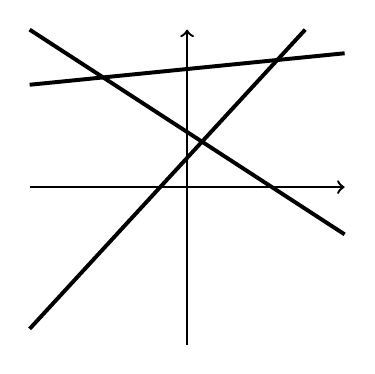
\begin{tikzpicture}
	\draw[line width=0.03cm,->] (-2,0) -- (2,0);
	\draw[line width=0.03cm,->] (0,-2) -- (0,2);
	\draw[line width= 0.05cm] (-2,1.3) -- (2,1.7);
	\draw[line width= 0.05cm] (-2,2) -- (2,-0.6);
	\draw[line width= 0.05cm] (-2,-1.8) -- (1.5,2);
	\end{tikzpicture}
	\qquad \qquad
	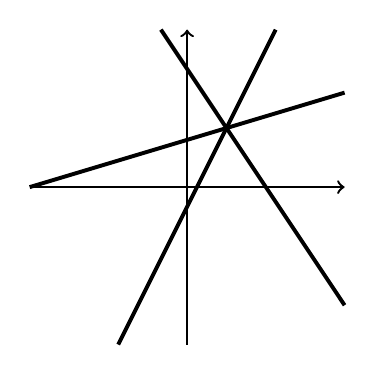
\begin{tikzpicture}
	\draw[line width=0.03cm,->] (-2,0) -- (2,0);
	\draw[line width=0.03cm,->] (0,-2) -- (0,2);
	\draw[line width= 0.05cm] (1.125, 2) -- (-0.875,-2);
	\draw[line width= 0.05cm] (-2,0) -- (2,1.2);
	\draw[line width= 0.05cm] (2,-1.5) -- (-0.333,2);
	\end{tikzpicture}
	\]



\newpage



% Quiz 16
\quizsol \textit{True/False}: The quadratic function $f(x)= 6 - (x + 2)^2$ is convex and has vertex $(2, 6)$. \pspace

\sol The statement is \textit{false}. The vertex form of a quadratic function $f(x)= ax^2 + bx + c$ is $f(x)$ written in the form $f(x)= a_0(x - P)^2 + Q$, where $a_0= a$ and $(P, Q)$ is the vertex of $f(x)$. Observe that $f(x)= 6 - (x + 2)^2= -(x + 2)^2 + 6= -\big(x - (-2) \big)^2 + 6$. But then $(P, Q)= (-2, 6)$, so that the vertex is $(-2, 6)$, and $a= -1 < 0$. We know a quadratic function $f(x)= ax^2 + bx + c$ is convex if $a > 0$ and is concave if $a < 0$. Therefore, $f(x)$ is a quadratic function with vertex $(-2, 6)$ and is concave. The given statement incorrectly identifies the $x$-coordinate of the vertex as $2$, rather than $-2$ (the $x$-value that makes the $(x + 2)^2$ term vanish) and also mistakes $a= 1$ rather than $a= -1$ so that the quadratic function is identified as being convex rather than concave. \pvspace{1.3cm}



% Quiz 17
\quizsol \textit{True/False}: Let $ax^2 + bx + c$ be a quadratic function. If $x_0= -\frac{b}{2a}$, then the vertex occurs at $\big(x_0, f(x_0) \big)$ and the minimum or maximum output of $f(x)$ is $f(x_0)$---depending on the value of $a$. \pspace

\sol The statement is \textit{true}. The location of the vertex is given by $x_0= -\frac{b}{2a}$. The $y$-coordinate of the vertex must be given by the function value at $x_0$ which is $f(x_0)$. But then the vertex is $\big(x_0, f(x_0) \big)$. We know that the $y$-coordinate of the vertex is the either the minimum or maximum output of $f$ depending on whether $f$ opens upwards or downwards, respectively. If $a > 0$, then the parabola opens upwards and $f(x_0)$ is a minimum. If $a < 0$, then the parabola opens downwards and $f(x_0)$ is a maximum. We can see that the vertex is $\big(x_0, f(x_0) \big)$ via the following argument: note that
	\[
	\begin{aligned}
	f(x_0)&= f \left(-\frac{b}{2a} \right) \\ 
	&= a \left(-\frac{b}{2a} \right)^2 + b \left(-\frac{b}{2a} \right) + c \\
	&= a \cdot \dfrac{b^2}{4a^2} - \dfrac{b^2}{2a} + c \\
	&= \dfrac{b^2}{4a} - \dfrac{b^2}{2a} + c \\
	&= \dfrac{b^2}{4a} - \dfrac{2b^2}{4a} + \dfrac{4ac}{4a} \\
	&= \dfrac{b^2 - 2b^2 + 4ac}{4a} \\
	&= \dfrac{-b^2 + 4ac}{4a} \\
	&= \dfrac{4ac - b^2}{4a}
	\end{aligned}
	\]
But then we have\dots
	\[
	\begin{aligned}
	ax^2 + bx + c&= a \left(x^2 + \dfrac{b}{a} \,x + \dfrac{c}{a} \right) \\
	&= a \left(x^2 + \dfrac{b}{a} \,x + \dfrac{b^2}{2^2a^2} - \dfrac{b^2}{2^2a^2} + \dfrac{c}{a} \right) 
	\end{aligned}
	\]
	\[
	\begin{aligned}
	&= a \left( \left(x + \dfrac{b}{2a} \right)^2 - \dfrac{b^2}{2^2a^2} + \dfrac{c}{a} \right) \\
	&= a \left(x + \dfrac{b}{2a} \right)^2 - \dfrac{b^2}{2^2a} + c \\
	&= a \left(x - \dfrac{-b}{2a} \right)^2 - \dfrac{b^2}{4a} + c \\
	&= a \left(x - \dfrac{-b}{2a} \right)^2 - \dfrac{b^2}{4a} + \dfrac{4ac}{4a} \\
	&= a \left(x - \dfrac{-b}{2a} \right)^2 + \dfrac{4ac - b^2}{4a} \\
	&= a \left(x - \dfrac{-b}{2a} \right)^2 + f(x_0)
	\end{aligned}
	\]
We see that this is the vertex form of the quadratic function $f(x)$ with vertex $(-\frac{b}{2a}, f(x_0))= \big(x_0, f(x_0) \big)$. \pvspace{1.3cm}



% Quiz 18
\quizsol \textit{True/False}: Let $f(x)= ax^2 + bx + c$ be a quadratic function. There will only be a distinct solution to the equation $f(x)= 0$ if the discriminant of $f(x)$ is zero. \pspace

\sol The statement is \textit{true}. Recall that the discriminant of a quadratic function $f(x)= ax^2 + bx + c$ is $D= b^2 - 4ac$. If $D < 0$, then $f(x)$ has two distinct, complex solutions. If $D > 0$, then $f(x)$ has two distinct real solutions. If $D= 0$, then $D$ has one distinct, rational solution. The exact solution(s) to a quadratic function are given by the quadratic formula:
	\[
	x= \dfrac{-b \pm \sqrt{b^2 - 4ac}}{2a}= \dfrac{-b \pm \sqrt{D}}{2a}
	\]
From the quadratic formula, we can also see that the nature of the roots depends only on $D$:
	\[
	\begin{aligned}
	D < 0&\colon x= \dfrac{-b \pm \sqrt{D}}{2a} \Longrightarrow x= \dfrac{-b \pm \sqrt{|D|} \, i}{2a}= \dfrac{-b}{2a} \pm \dfrac{\sqrt{|D|}}{2a} \, i \\[0.3cm]
	D > 0&\colon x= \dfrac{-b \pm \sqrt{D}}{2a} \Longrightarrow x= \dfrac{-b}{2a} \pm \dfrac{1}{2a} \, \sqrt{D} \\[0.3cm]
	D= 0&\colon x= \dfrac{-b \pm \sqrt{D}}{2a} \Longrightarrow x= \dfrac{-b}{2a}
	\end{aligned}
	\] \pvspace{1.3cm}



% Quiz 19
\quizsol \textit{True/False}: For any polynomial $ax^2 + bx + c$, there exists a factorization $(x - r_1)(x - r_2)$, where $r_1, r_2$ are rational numbers. \pspace

\sol The statement is \textit{false}. Observe that there can never be an expression of the form $(x - r_1)(x - r_2)$ for the quadratic function $2x^2 + 3x + 1$ because $a= 2$ while $(x - r_1)(x - r_2)= x^2 - (r_1 + r_2)x + r_1r_2$ has $a= 1$. Furthermore, if every quadratic function could be expressed as $(x - r_1)(x - r_2)$, every quadratic function would have rational roots $r_1, r_2$. However, we know that not all quadratic functions have rational roots---or even real roots. We can determine the nature of the roots from the discriminant of $ax^2 + bx + c$, which is $D= b^2 - 4ac$. If $D < 0$, then $f(x)$ has two distinct, complex solutions. If $D > 0$, then $f(x)$ has two distinct real solutions. If $D= 0$, then $D$ has one distinct, rational solution. Therefore, the polynomial $ax^2 + bx + c$ will have an expression of the form $(x - r_1)(x - r_2)$ if and only if $D > 0$ and $a= 1$. 






A polynomial of degree 10 can have five distinct zeros with exactly two of those roots having multiplicity at least three.

















\end{document}